% Template for PLoS
% Version 3.1 February 2015
%
% To compile to pdf, run:
% latex plos.template
% bibtex plos.template
% latex plos.template
% latex plos.template
% dvipdf plos.template
%
% % % % % % % % % % % % % % % % % % % % % %
%
% -- IMPORTANT NOTE
%
% This template contains comments intended 
% to minimize problems and delays during our production 
% process. Please follow the template instructions
% whenever possible.
%
% % % % % % % % % % % % % % % % % % % % % % % 
%
% Once your paper is accepted for publication, 
% PLEASE REMOVE ALL TRACKED CHANGES in this file and leave only
% the final text of your manuscript.
%
% There are no restrictions on package use within the LaTeX files except that 
% no packages listed in the template may be deleted.
%
% Please do not include colors or graphics in the text.
%
% Please do not create a heading level below \subsection. For 3rd level headings, use \paragraph{}.
%
% % % % % % % % % % % % % % % % % % % % % % %
%
% -- FIGURES AND TABLES
%
% Please include tables/figure captions directly after the paragraph where they are first cited in the text.
%
% DO NOT INCLUDE GRAPHICS IN YOUR MANUSCRIPT
% - Figures should be uploaded separately from your manuscript file. 
% - Figures generated using LaTeX should be extracted and removed from the PDF before submission. 
% - Figures containing multiple panels/subfigures must be combined into one image file before submission.
% For figure citations, please use "Fig." instead of "Figure".
% See http://www.plosone.org/static/figureGuidelines for PLOS figure guidelines.
%
% Tables should be cell-based and may not contain:
% - tabs/spacing/line breaks within cells to alter layout or alignment
% - vertically-merged cells (no tabular environments within tabular environments, do not use \multirow)
% - colors, shading, or graphic objects
% See http://www.plosone.org/static/figureGuidelines#tables for table guidelines.
%
% For tables that exceed the width of the text column, use the adjustwidth environment as illustrated in the example table in text below.
%
% % % % % % % % % % % % % % % % % % % % % % % %
%
% -- EQUATIONS, MATH SYMBOLS, SUBSCRIPTS, AND SUPERSCRIPTS
%
% IMPORTANT
% Below are a few tips to help format your equations and other special characters according to our specifications. For more tips to help reduce the possibility of formatting errors during conversion, please see our LaTeX guidelines at http://www.plosone.org/static/latexGuidelines
%
% Please be sure to include all portions of an equation in the math environment.
%
% Do not include text that is not math in the math environment. For example, CO2 will be CO\textsubscript{2}.
%
% Please add line breaks to long display equations when possible in order to fit size of the column. 
%
% For inline equations, please do not include punctuation (commas, etc) within the math environment unless this is part of the equation.
%
% % % % % % % % % % % % % % % % % % % % % % % % 
%
% Please contact latex@plos.org with any questions.
%
% % % % % % % % % % % % % % % % % % % % % % % %

\documentclass[10pt,letterpaper,draft]{article}
\usepackage[top=0.85in,left=2.75in,footskip=0.75in]{geometry}

% Use adjustwidth environment to exceed column width (see example table in text)
\usepackage{changepage}

% Use Unicode characters when possible
\usepackage[utf8]{inputenc}

% textcomp package and marvosym package for additional characters
\usepackage{textcomp,marvosym}

% fixltx2e package for \textsubscript
\usepackage{fixltx2e}

% amsmath and amssymb packages, useful for mathematical formulas and symbols
\usepackage{amsmath,amssymb}

% cite package, to clean up citations in the main text. Do not remove.
\usepackage{cite}

% Use nameref to cite supporting information files (see Supporting Information section for more info)
\usepackage{nameref,hyperref}

% line numbers
\usepackage[right]{lineno}

% ligatures disabled
\usepackage{microtype}
\DisableLigatures[f]{encoding = *, family = * }

% rotating package for sideways tables
\usepackage{rotating}

% Remove comment for double spacing
\usepackage{setspace} 
\doublespacing

% Text layout
\raggedright
\setlength{\parindent}{0.5cm}
\textwidth 5.25in 
\textheight 8.75in

% Bold the 'Figure #' in the caption and separate it from the title/caption with a period
% Captions will be left justified
\usepackage[aboveskip=1pt,labelfont=bf,labelsep=period,justification=raggedright,singlelinecheck=off]{caption}

% Use the PLoS provided BiBTeX style
\bibliographystyle{plos2015}

% Remove brackets from numbering in List of References
\makeatletter
\renewcommand{\@biblabel}[1]{\quad#1.}
\makeatother

% Leave date blank
\date{}

% Header and Footer with logo
\usepackage{lastpage,fancyhdr,graphicx}
\usepackage{epstopdf}
\pagestyle{myheadings}
\pagestyle{fancy}
\fancyhf{}
\lhead{
\includegraphics[width=2.0in]{PLOS-submission.eps}}
\rfoot{\thepage/\pageref{LastPage}}
\renewcommand{\footrule}{\hrule height 2pt \vspace{2mm}}
\fancyheadoffset[L]{2.25in}
\fancyfootoffset[L]{2.25in}
\lfoot{\sf PLOS}

%% Include all macros below

\newcommand{\lorem}{{\bf LOREM}}
\newcommand{\ipsum}{{\bf IPSUM}}

%% END MACROS SECTION


%%%% Additional user-defined macros

%% Math

% Operators
\DeclareMathOperator{\Cov}{Cov}
\DeclareMathOperator{\Var}{Var}
\DeclareMathOperator{\E}{\mathbb{E}}
\DeclareMathOperator{\Proba}{\mathbb{P}}

\newcommand{\Covb}[2]{\ensuremath{\Cov\!\left[#1,#2\right]}}
\newcommand{\Eb}[1]{\ensuremath{\E\!\left[#1\right]}}
\newcommand{\Pb}[1]{\ensuremath{\Proba\!\left[#1\right]}}
\newcommand{\Varb}[1]{\ensuremath{\Var\!\left[#1\right]}}

% norm
\newcommand{\norm}[1]{\| #1 \|}


\usepackage{ragged2e}




\begin{document}
\vspace*{0.35in}

% Title must be 250 characters or less.
% Please capitalize all terms in the title except conjunctions, prepositions, and articles.
\begin{flushleft}
{\Large\textbf\newline{
Calibration of a Density-based Model of Urban Morphogenesis
}
}
\newline
% Insert author names, affiliations and corresponding author email (do not include titles, positions, or degrees).
\\
Raimbault Juste\textsuperscript{1,2,*}
\\
\bigskip
\bf{1} UMR CNRS 8504 G{\'e}ographie-cit{\'e}s, Paris, France
\\
\bigskip
\bf{2} UMR-T 9403 IFSTTAR LVMT, Champs-sur-Marne, France

% Insert additional author notes using the symbols described below. Insert symbol callouts after author names as necessary.
% 
% Remove or comment out the author notes below if they aren't used.
%
% Primary Equal Contribution Note
%\Yinyang These authors contributed equally to this work.

% Additional Equal Contribution Note
% Also use this double-dagger symbol for special authorship notes, such as senior authorship.
%\ddag These authors also contributed equally to this work.

% Current address notes
%\textcurrency a Insert current address of first author with an address update
% \textcurrency b Insert current address of second author with an address update
% \textcurrency c Insert current address of third author with an address update

% Deceased author note
%\dag Deceased

% Group/Consortium Author Note
%\textpilcrow Membership list can be found in the Acknowledgments section.

% Use the asterisk to denote corresponding authorship and provide email address in note below.
* Corresponding Author

Email : juste.raimbault@polytechnique.edu

\end{flushleft}
% Please keep the abstract below 300 words
\begin{abstract}
\justify
We propose a stochastic model of urban growth that generates spatial distributions of population densities, at an intermediate scale between economic models at the macro scale and land-use evolution models focusing on local relations. Integrating simply the two opposite key processes of aggregation (``preferential attachment'') and diffusion (urban sprawl), we show that we can capture the whole spectrum of existing urban forms in Europe. An extensive exploration and calibration of the proposed model allows determining the region of parameter space corresponding morphologically to observed european urban systems, providing an validated thematic interpretation to model parameters, and furthermore determining the effective dimension of the urban system at this scale regarding morphological objectives.
\end{abstract}



\linenumbers


% http://journals.plos.org/plosone/article/file?id=10.1371/journal.pone.0166960&type=printable
%  -> good example of short abmodeling plosone paper (on extended schelling model).

\justify


%%%%%%%%%%%%%%%%%%%%%%%%
\section*{Introduction}


Urban Systems are complex socio-technical systems which can be studied from a large variety of viewpoints and disciplines: Batty has advocated in that sense for the construction of a dedicated science defined by its objects of study more than the methods used~\cite{batty2013new}. Simulating urban growth is one typical aspect 
As the short term trend is towards a mostly urbanized 

% ⇒ Plus réponse à cette question : pourquoi simuler la croissance urbaine (quels enjeux scientifiques et sociaux ?)


% - > literature on stochastic urban growth, ABM for Urban Growth, CA Models and urban morphogenesis models. Reproducing urban growth at different scales, capturing different processes.

% Macro models (Gibrat and extensions) are partially spatialized (Favaro - Pumain includes distance between cities, Simpops/Marius also) whereas micro (most CA) are ‘’over-spatialized’’ (neighborhood-based).  
% -> Research Question :  What about a simple model at the meso scale, close to macro by the stylized facts (preferential attachment) but producing morphologically consistent spatial distribution of densities ?



\cite{andersson2002urban} propose a micro-based model of urban growth, with the purpose to replace non-interpretable physical mechanisms with agent mechanisms, including interactions forces and mobility choices. Local correlations are used in \cite{makse1998modeling}, which develops the model introduced in~\cite{makse1995modelling},  to modulate growth patterns to ressemble real configurations. 

\cite{courtat2011mathematics} morphogenesis for roads

Cellular automata \cite{ward2000stochastically} \cite{GEAN:GEAN940}


\cite{frankhauser1998fractal}

In the same spirit, our model situates at similar scales and can be qualified as a morphogenesis model.



The rest of this paper is organized as follows: we first describe formally the model and the morphological indicators; we then develop results of real morphological measures, model exploration and model calibration.


%%%%%%%%%%%%%%%%%%%%%%%%
\section*{Material and Methods}
%%%%%%%%%%%%%%%%%%%%%%%%


%%%%%%%%%%%%%%%%%%%%%%%%
\subsection*{Urban growth model}
%%%%%%%%%%%%%%%%%%%%%%%%



%%%%%%%%%%%%%%%%%%%%%%%%
\paragraph*{Rationale}



%Preferential attchment and diffusion, extension of [Batty, 2006]. small litt. prefAtt and then Urban sprawl, opposed forces that must shape morphology of urban systems. choice of a scale at which spatial form has a sense but city system is ‘’wide enough” : 50-100km, meso-scale ?


\cite{2016arXiv160806313S} : how Simon model generates power law (paper more general to be quoted ?) ; first mover : path dependency of obtained shapes.



Our model is based on widely accepted ideas of diffusion-aggregation processes for Urban Processes. The combination of attraction forces with repulsion, due for example to congestion, already yield a complex outcome that has been shown under some simplifying assumptions to be representative of urban growth processes. Such a model is studied by~\cite{batty2006hierarchy}. Indeed, the tension between antagonist aggregation and sprawl mechanisms may be an important process in urban morphogenesis. For example \cite{fujita1996economics} opposes centrifugal forces with centripetal forces in the equilibrium view of urban spatial systems, what is easily transferable to non-equilibrium systems in the framework of self-organized complexity : a urban structure is a far-from-equilibrium system that has been driven to this point by these opposite forces. The two contradictory processes of urban concentration and urban sprawl are captured by the model, what allows to reproduce with a good precision a large number of existing morphologies.



% choice of scale : linked to the notion of morphogenesis

The question at which scale is it possible and relevant to define and try to simulate urban form is rather open, and will in fact depend on which issues are being tackled. 




\paragraph*{Formalization}



We formalize now the model, together with its parameters and their possible interpretations. The simulation model proceeds iteratively the following way. The world is a square grid of width $N$, in which each cell is characterized by its population $(P_i(t))_{1\leq i\leq N^2}$. initially empty, is represented . At each time step, until total population reaches a fixed parameter $P_m$,

\begin{itemize}
\item total population is increased of a fixed number $N_G$ (growth rate), following a preferential attachment such that 
\[\Pb{P_i(t+1)=P_i(t)+1|P(t+1)=P(t)+1}=\frac{(P_i(t)/P(t))^{\alpha}}{\sum(P_i(t)/P(t))^{\alpha}}\]
\item a fraction $\beta$ of population is diffused to cell neighborhood, this operation being repeated $n_d$ times
\end{itemize}





\paragraph*{Indicators}


% Literature on morphological analysis, method taken from [Le Nechet 2015] to qualify/quantify urban form. Why would form be relevant at this scale ? -> thematic references on variety of urban developments, rural settlements, etc. : form translates many spatial processes at this scale. [beware question of equifiniality : model is however themtically-based for processes].

\cite{guerois2008built} : sort of morphological analysis


% on other ways to quantify form ? -> ex fractal shape index ; recent research \cite{2016arXiv160808839C}


As our model is only density-based, we propose to quantify its outputs through spatial morphology, i.e. characteristics of density spatial distribution. We need therefore quantities having a certain level of robustness and invariance. For example, two polycentric cities should be classified as morphologically close whereas a direct comparison of distributions (Earth Mover Distance e.g.) could give a very high distance between configurations depending on center positions. To tackle this issue, we refer to the Urban Morphology Analysis literature which proposes an extensive set of indicators to describe urban form~\cite{tsai2005quantifying}. The number of dimensions can be reduced to obtain a robust description with a few number of independent indicators~\cite{Schwarz201029}. For the choice of indicators, we follow the analysis done in~\cite{le2015forme} where a typology of large european cities is obtained in consistence with qualitative knowledge. Let denote $(P_i)_{1\leq i \leq N}$ the population of cells, sorted in decreasing order, $d_{ij}$ the distance between cells $i,j$, and $P=\sum_{i=1}^{N} P_i$ total population. The indicators are the following :

\begin{enumerate}
\item Rank-size slope $\gamma$, expressing the degree of hierarchy in the distribution, computed by fitting with Ordinary Least Squares a power law distribution by $\ln{P_i/P_0} \sim k - \gamma\cdot \ln{i/i_0}$.
\item Distribution Entropy
\begin{equation}
\mathcal{E} = \sum_{i=1}^{N}\frac{P_i}{P}\cdot \ln{\frac{P_i}{P}}
\end{equation}
\item Spatial-autocorrelation given by Moran index, with simple spatial weights given by $w_{ij} = 1/d_{ij}$
\[
r = \frac{\sum_{i\neq j} w_{ij} \left(P_i - \bar{P}\right)\cdot\left(P_j - \bar{P}\right)}{\sum_{i\neq j} w_{ij} \sum_{i}{\left( P_i - \bar{P}\right)}^2}
\]
\item Mean distance between individuals, which captures population concentration
\[
\bar{d} = \sum_{i<j} \frac{P_i P_j}{P^2} \cdot d_{ij}
\]
\end{enumerate}






%%%%%%%%%%%%%%%%%%%%%%%%
\subsection*{Real Data}

%% Data source (density grid), computation methodology [comparison of sampling/smoothing to avoid bord effects ?] -> reals values of morpho indics on 50kmx50km grids, on all Europe.
%% + summary stats

%Figure : Distributions of indicators values for real dataset of european densities, computed on 50kmx50km grids, with 10km offset to avoid bord effects. [TODO : add log-normal/normal fits ? ]
%  -> cf Empirical Section

We compute morphological measure on real urban density data, namely the population density grid of th European Union at 100m resolution provided openly by Eurostat~\cite{eurostat}. The morphological measures used for calibration are the one described above that are the same used to classify model outputs. The calibration of the model is thus done on morphological objectives (entropy, hierarchy, spatial auto-correlation, mean distance). We show in Fig.~\ref{fig:empirical} maps giving values of indicators for France, to ease readability. Maps for the full European union are available in~\nameref{S1_Text}. The choice of the resolution, the space range, and the shape of the window on which indicators are computed, is made according to the thematic specifications of the model : 
We however tested the sensitivity to window size and shape



%%%%%%%%%%%%%%%%%%%%%%%%
\begin{figure}
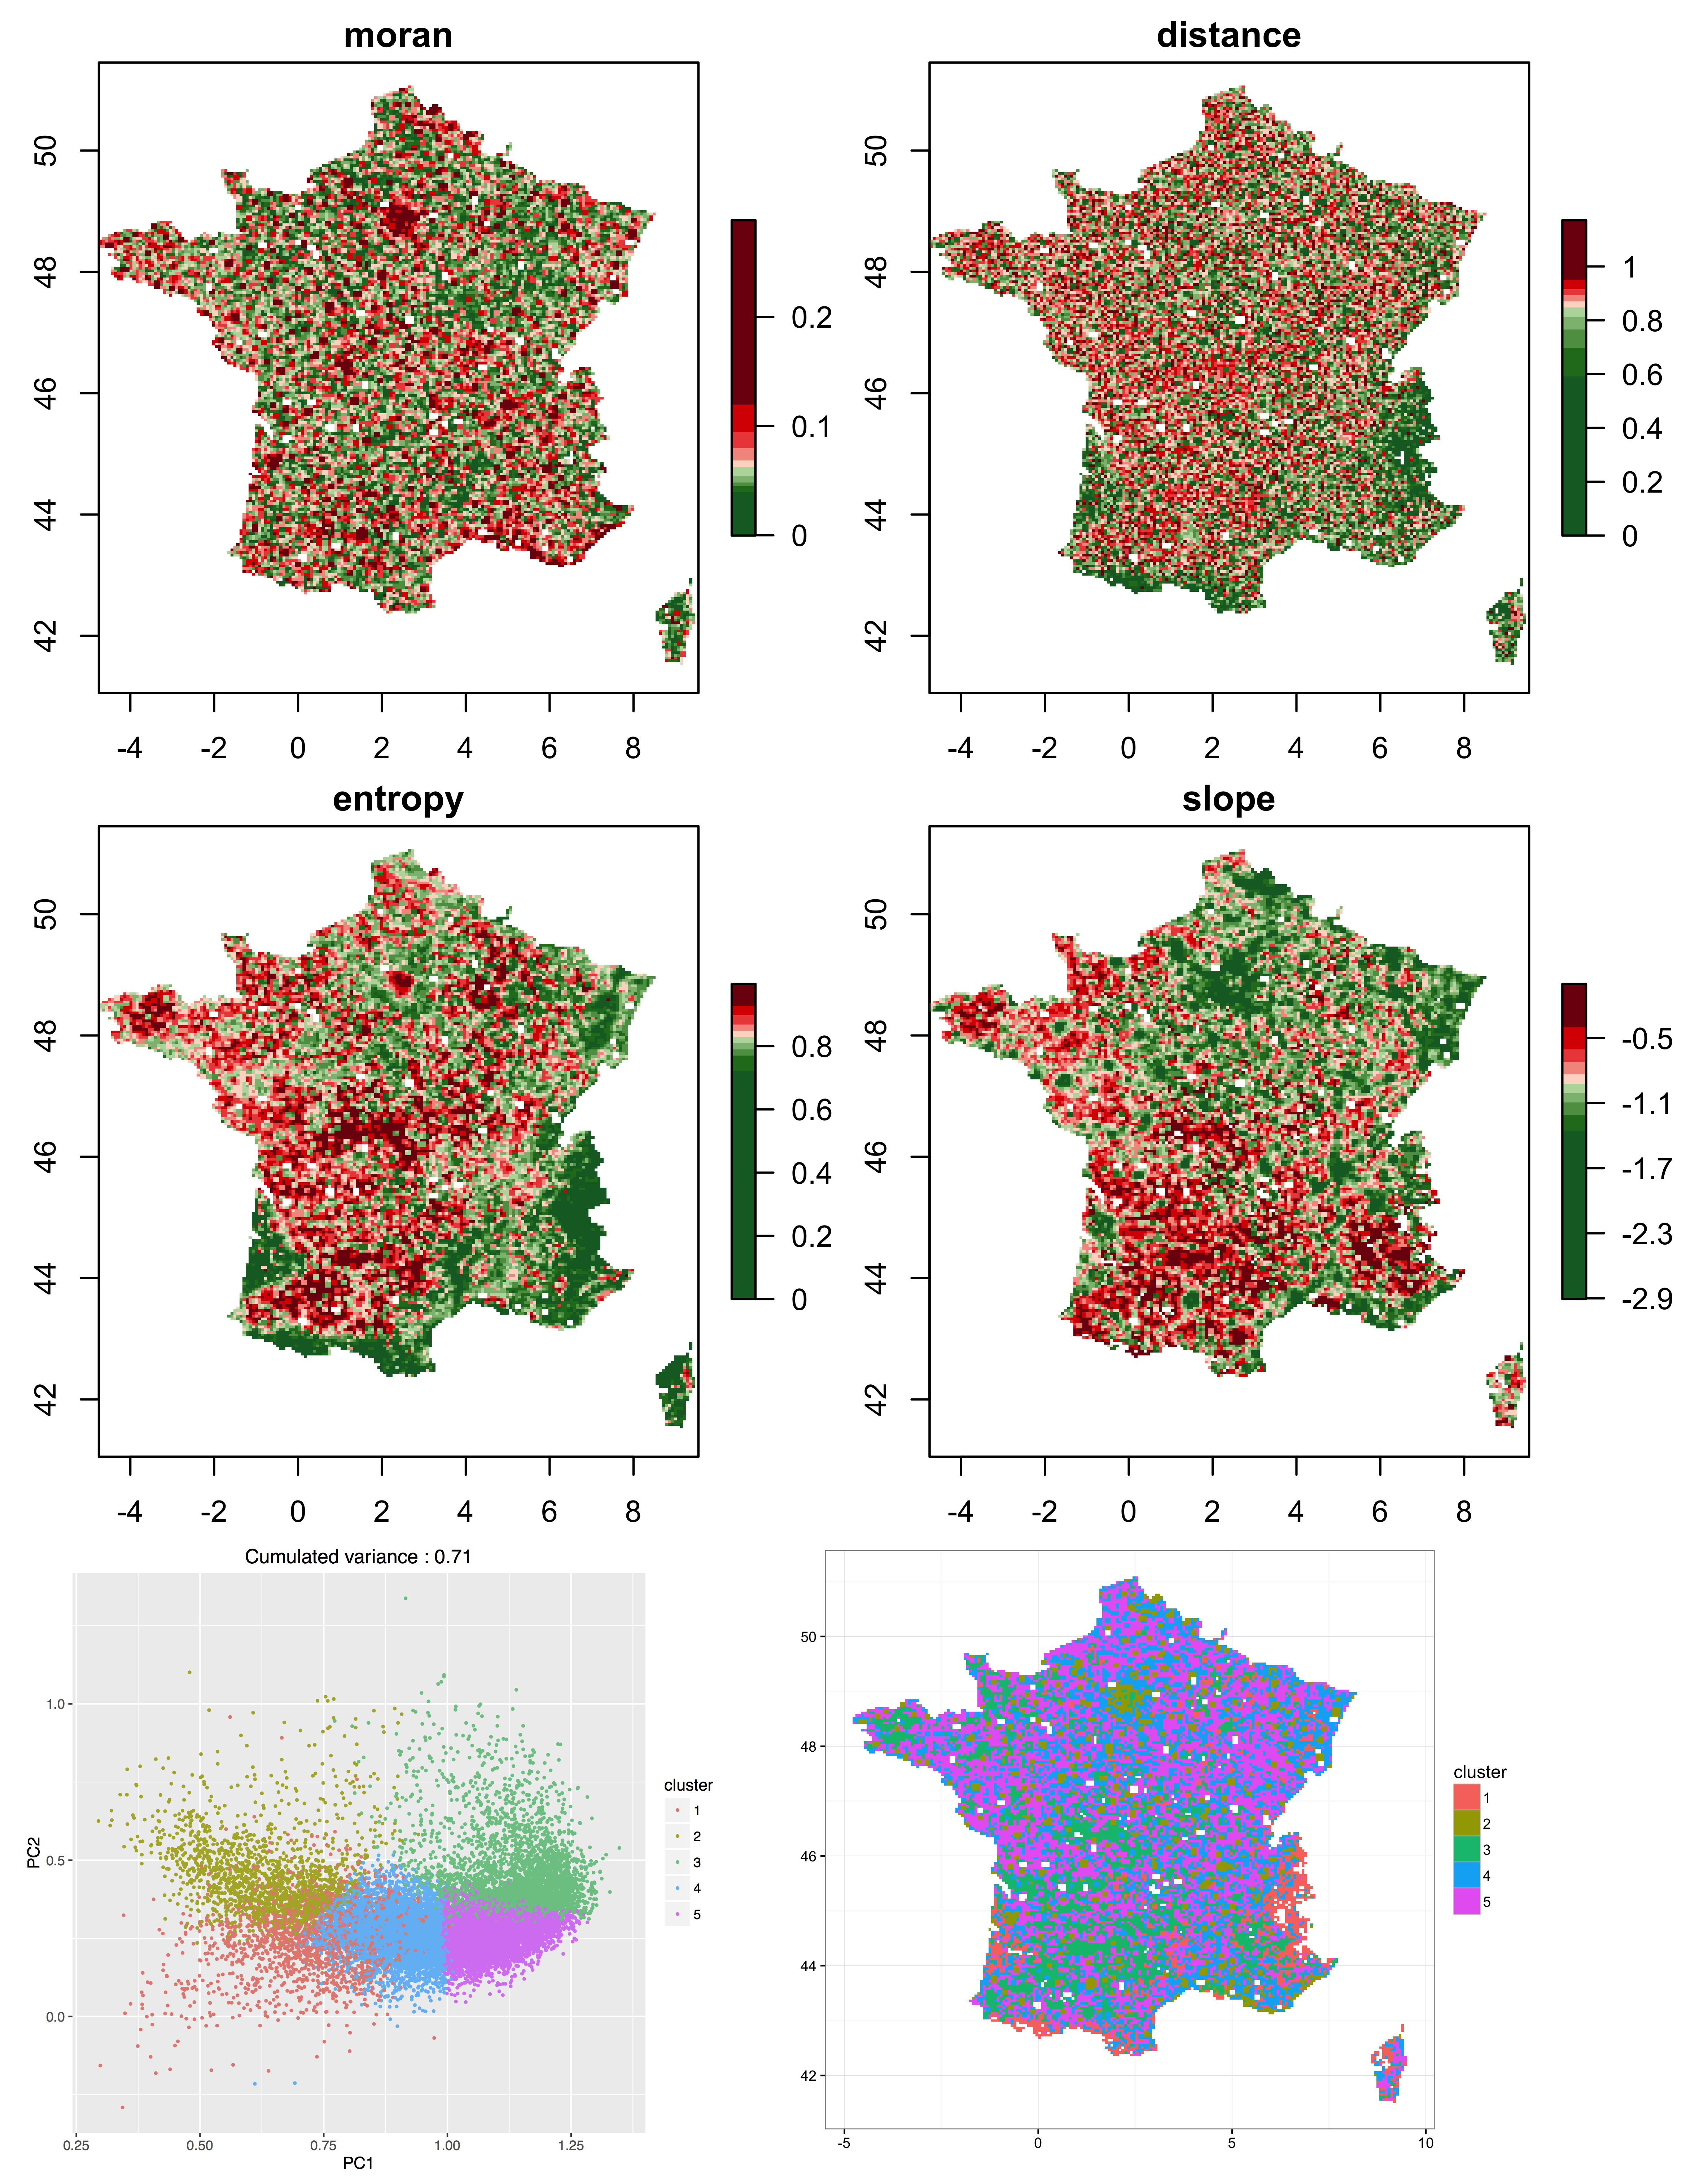
\includegraphics[width=\textwidth]{figures/Fig1.png}
%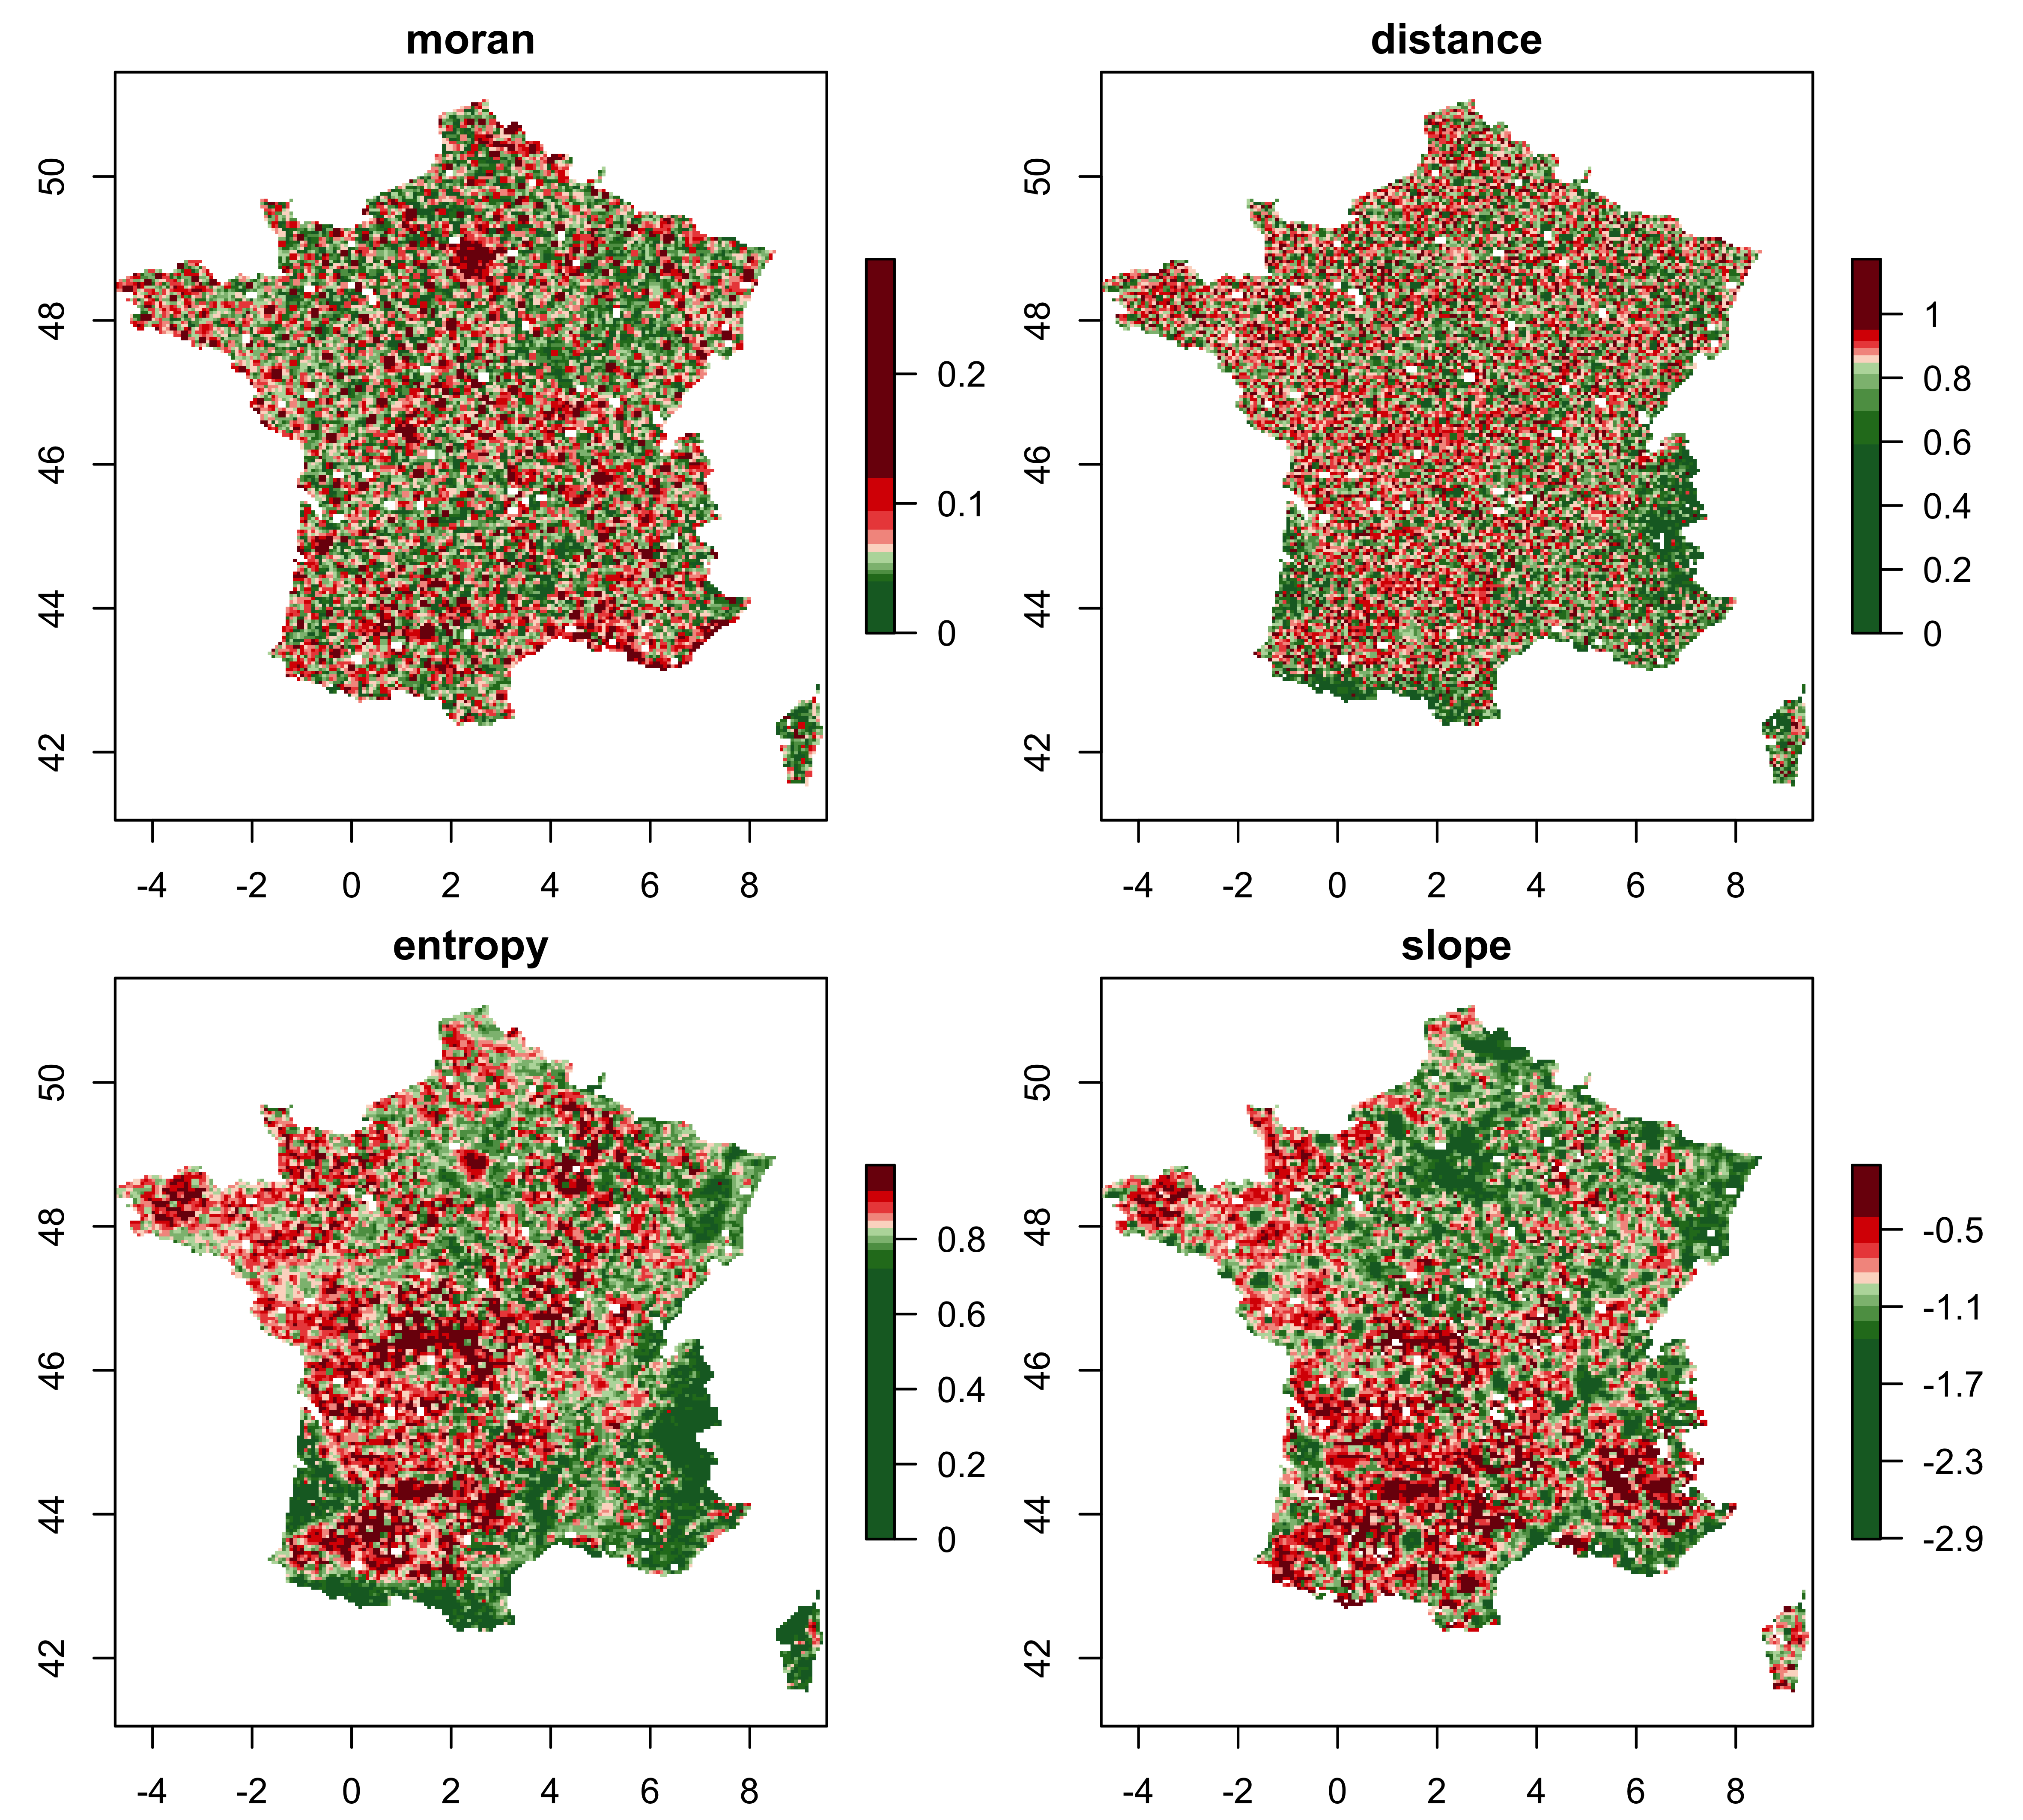
\includegraphics[width=\textwidth]{figures/indics_morpho_discrquantiles}\\
%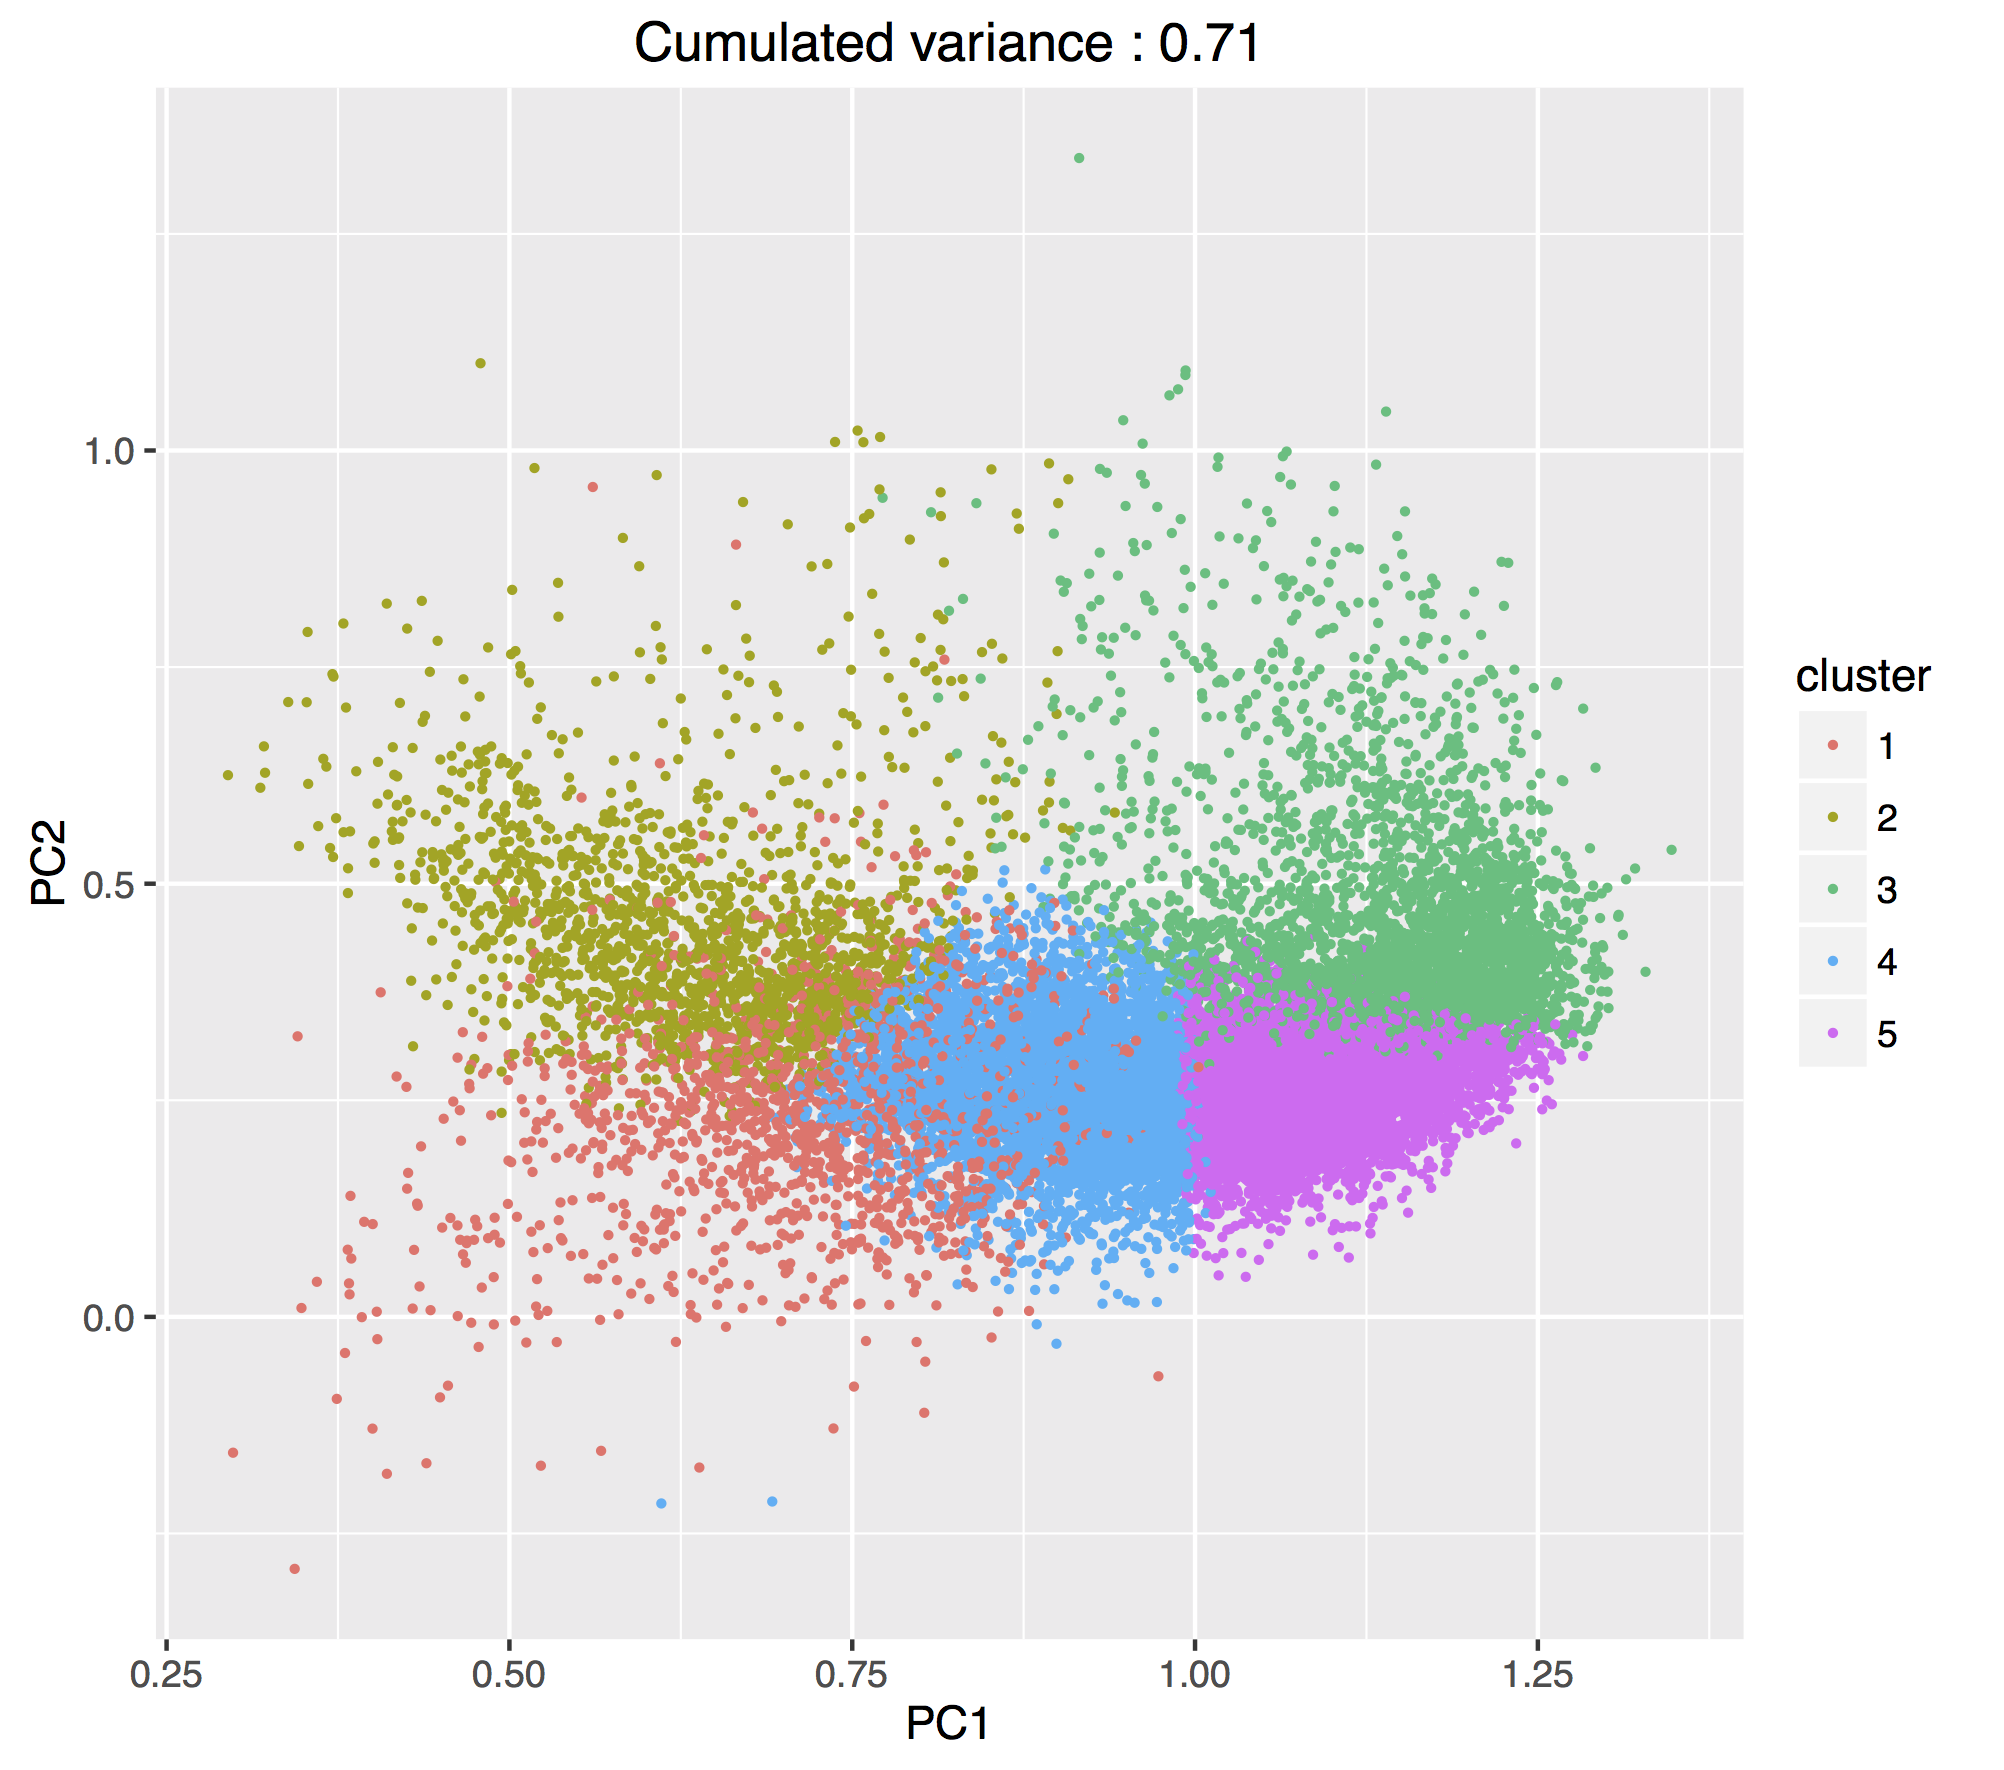
\includegraphics[width=0.49\textwidth]{figures/cluster_pca_k5_morpho}
%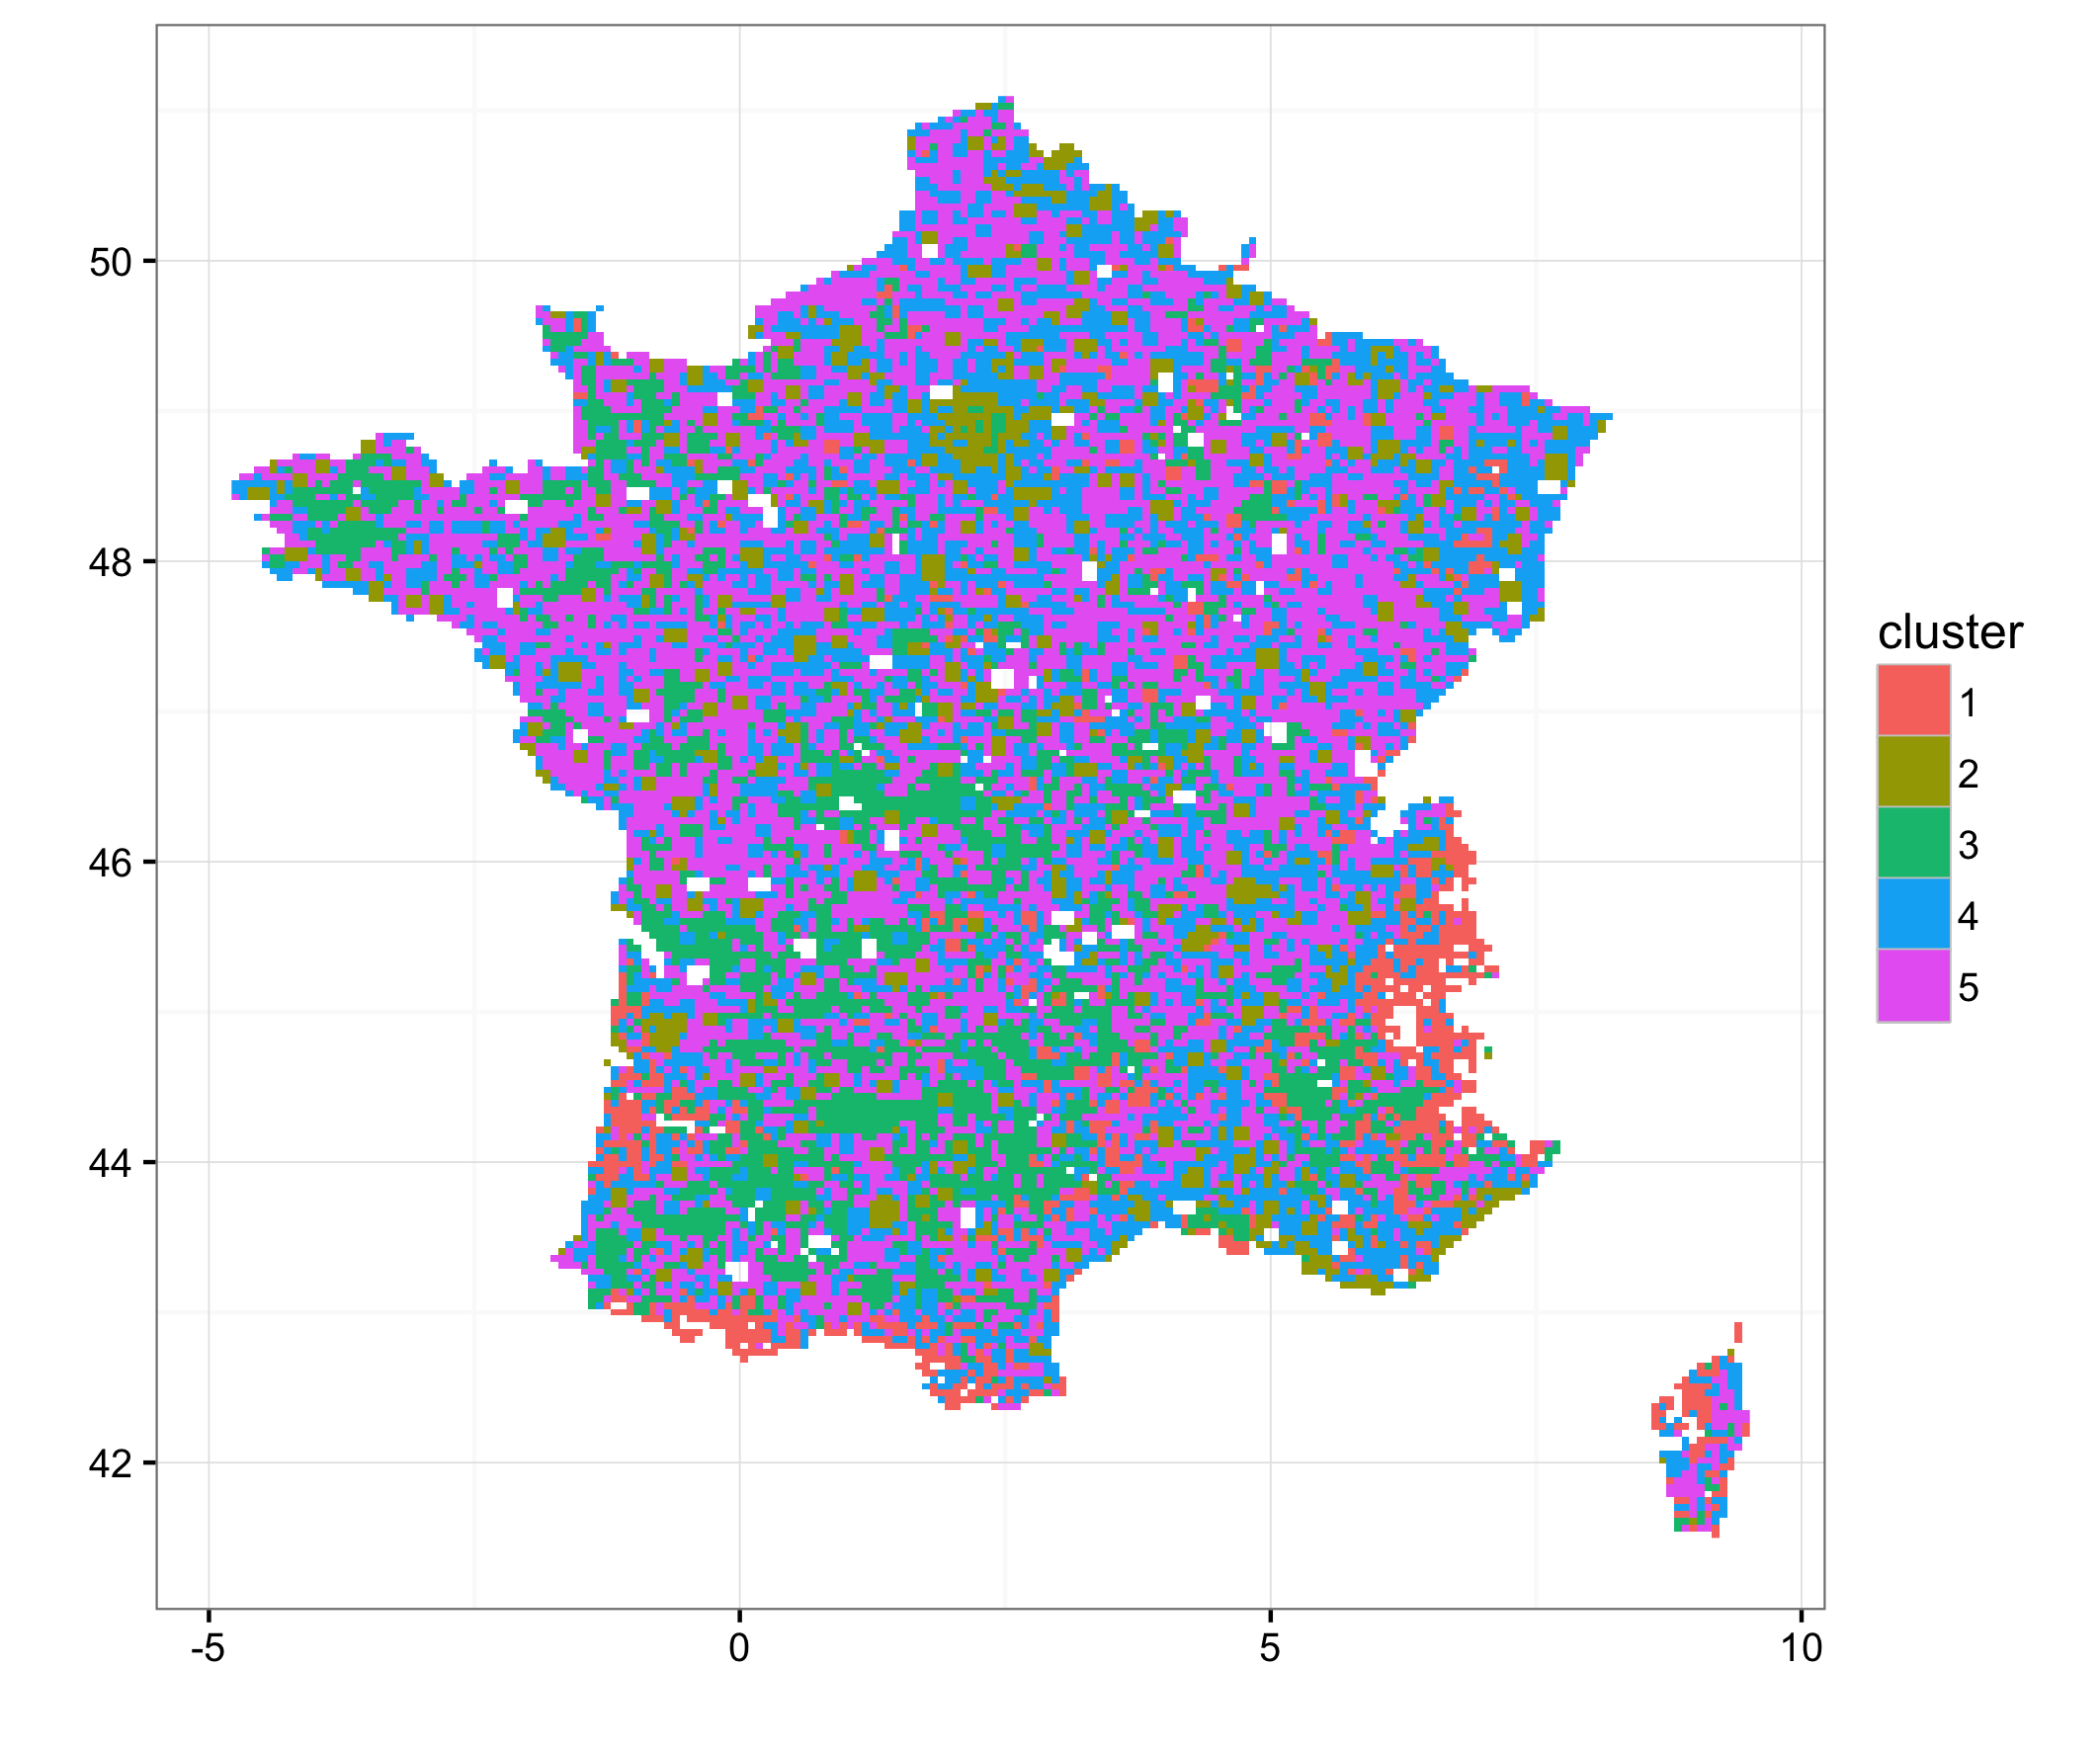
\includegraphics[width=0.49\textwidth]{figures/cluster_map_k5_morpho}
\caption{\textbf{Empirical values of morphological indicators.} }
\label{fig:empirical}
\end{figure}
%%%%%%%%%%%%%%%%%%%%%%%%











%%%%%%%%%%%%%%%%%%%%%%%%
\section*{Results}
%%%%%%%%%%%%%%%%%%%%%%%%





%%%%%%%%%%%%%%%%%%%%%%%%
\subsection*{Generation of urban patterns}


\paragraph{Implementation}


The model is implemented both in NetLogo~\cite{wilensky1999netlogo} for exploration and visualization purposes, and in \texttt{Scala} for performance reasons and easy integration into OpenMole~\cite{reuillon2013openmole}, which allows a transparent access to High Performance Computing environments. Computation of indicator values on geographical data is done in \texttt{R} using the \texttt{raster} package~\cite{hijmans2015geographic}. Source code and results are available on the open repository of the project at \texttt{https://github.com/JusteRaimbault/CityNetwork/tree/master/Models/Synthetic/Density}. Raw datasets for real indicator values and simulation results are available on Dataverse at \texttt{http://dx.doi.org/10.7910/DVN/WSUSBA}.



\paragraph{Generated Shapes}

The model has a relatively small number of parameters but is able to generate a very wide variety of shapes, extending beyond existing forms. In particular, its dynamical nature allows through $P_m$ parameter to choose final regime that can be non-stationarity (generally chaotic shapes), semi-stationarity or full stationarity. Fig.~\ref{fig:fig2} shows examples of generated shapes, and illustrates the variety of forms that can be produced by the model.




%%%%%%%%%%%%%
\begin{figure}
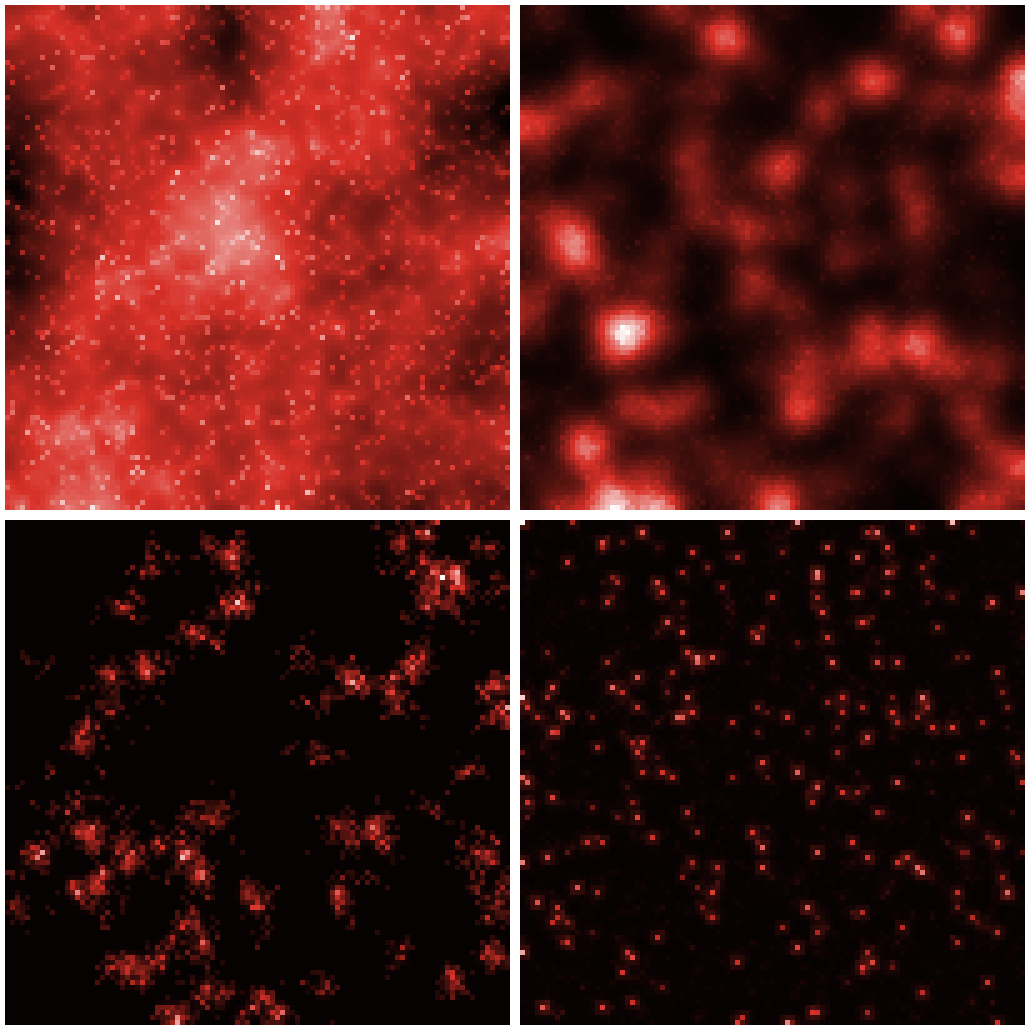
\includegraphics[width=\textwidth]{figures/Fig2.png}
%ex_sp-diffusion=0.05_sp-growth-rate=76_sp-diffusion-steps=2_sp-alpha-localization=0.4_ticks=995_sp-population=75620.00000000015.png
%ex_sp-diffusion=0.047_sp-growth-rate=274_sp-diffusion-steps=2_sp-alpha-localization=1.4_ticks=197_sp-population=53977.999999999935.png
%ex_sp-diffusion=0.0060_sp-growth-rate=25_sp-diffusion-steps=1_sp-alpha-localization=0.4_ticks=176_sp-population=4400.000000000003.png
%ex_sp-diffusion=0.0060_sp-growth-rate=268_sp-diffusion-steps=1_sp-alpha-localization=1.6_ticks=285_sp-population=76376.00000000033.png
\caption{\textbf{Example of the variety of generated urban shapes.}}
\label{fig:fig2}
\end{figure}
%%%%%%%%%%%%%




%%%%%%%%%%%%%%%%%%%%%%%%
\subsection*{Model Behavior}



In the study of such a computational model of simulation, the lack of analytical tractability must be balanced by an extensive knowledge of model behavior in the parameter space. 

%(pub openmole exploration etc, importance of intensive computation)

\paragraph{Convergence}


Indicators show good convergence property and bimodal statistical distribution for cumulated points in the parameter space confirm the existence of superposed regimes : gaussian distribution gives stationary configurations, whereas inverse log-normal distribution are close to real data shape and correspond to non-stationary regime. For one point and a large number of repetitions, we find that 50 repetitions are enough to obtain a 95\% confidence interval smaller than $\sigma$ around indicator mean. 



\paragraph{Exploration of parameter space}

We sample the Parameter space using a Latin Hypercube Sampling. Parameter bounds are $\alpha \in [0.2,2],\beta \in [0,0.1],n_d \in \{0,\ldots , 4\}, N_G \in [500,3000], P_m \in [2000,100000]$.




%%%%%%%%%%%%%
\begin{figure}
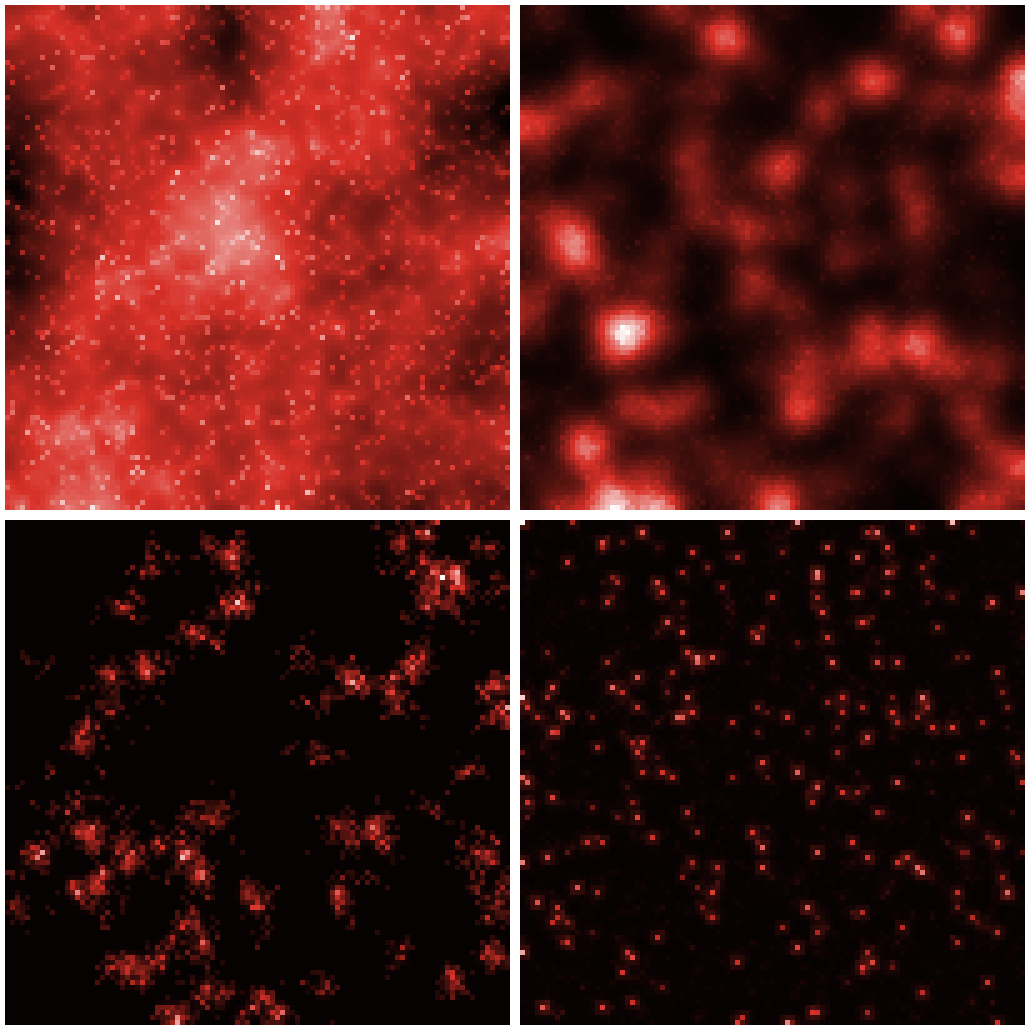
\includegraphics[width=\textwidth]{figures/Fig3.png}
\caption{\textbf{Behavior of indicators.}}
\label{fig:fig3}
\end{figure}
%%%%%%%%%%%%%






%%%%%%%%%%%%%%%%%%%%%%%%
\subsection*{Semi-analytical Analysis}\label{subsec:analytical}

Our model can be understood as a type of reaction-diffusion model, that have been widely used in other fields such as biology: similar processes were used for example by Turing in its seminal paper on morphogenesis~\cite{turing1952chemical}. An other way to formulate the model typical to these approaches is by using Partial Differential Equations. We propose to gain insights into long-time dynamics by studying them on a simplified case. We consider the system in one dimension, such that $x\in \left[0;1\right]$ with $1/\delta x$ cells of size $\delta x$. Each cell is characterized by its population as a random variable $P(x,t)$. We work on their expected values $p(x,t) = \Eb{P(x,t)}$, and assume that $n_d=1$. As developed in Supplementary Material~\nameref{S2_Text}, we show that this simplified process verifies the following PDE:

\begin{equation}\label{eq:pde}
\delta t \cdot \frac{\partial p}{\partial t} = \frac{N_G \cdot p^{\alpha-2}}{P_{\alpha}(t)}\cdot \left(p^2 + \frac{\alpha \beta \delta x^2}{2}\cdot \left[ \frac{\partial^2 p}{\partial x^2} \cdot p + (\alpha - 1) \left(\frac{\partial p}{\partial x}\right)^2 \right] \right) - p
\end{equation}


We learn the following properties:
\begin{enumerate}
\item Existence of a stationary solution for population proportion
\item Characteristic distance of the stationary distribution
\item Existence of bifurcations in the random case
\end{enumerate}

% thus the model must be used in a non-stationary way in time and space, $\gamma = P_m / N_G$ is crucial.




%%%%%%%%%%%%%%%%%%%%%%%%
\subsection*{Model Calibration}



We use a specific calibration process: a principal component analysis allows to maximize the cumulated distance between generated points and reals points. We select then the point cloud that overlaps real points in the (PC1,PC2) plan, given a distance threshold. Fig.~\ref{fig:densitycalib} shows the points we obtain for four different values of the threshold ranging from $10^{-6}$ to $10^{-3}$.




%%%%%%%%%%%%%%%
\begin{figure}
%\hspace{-2cm}
%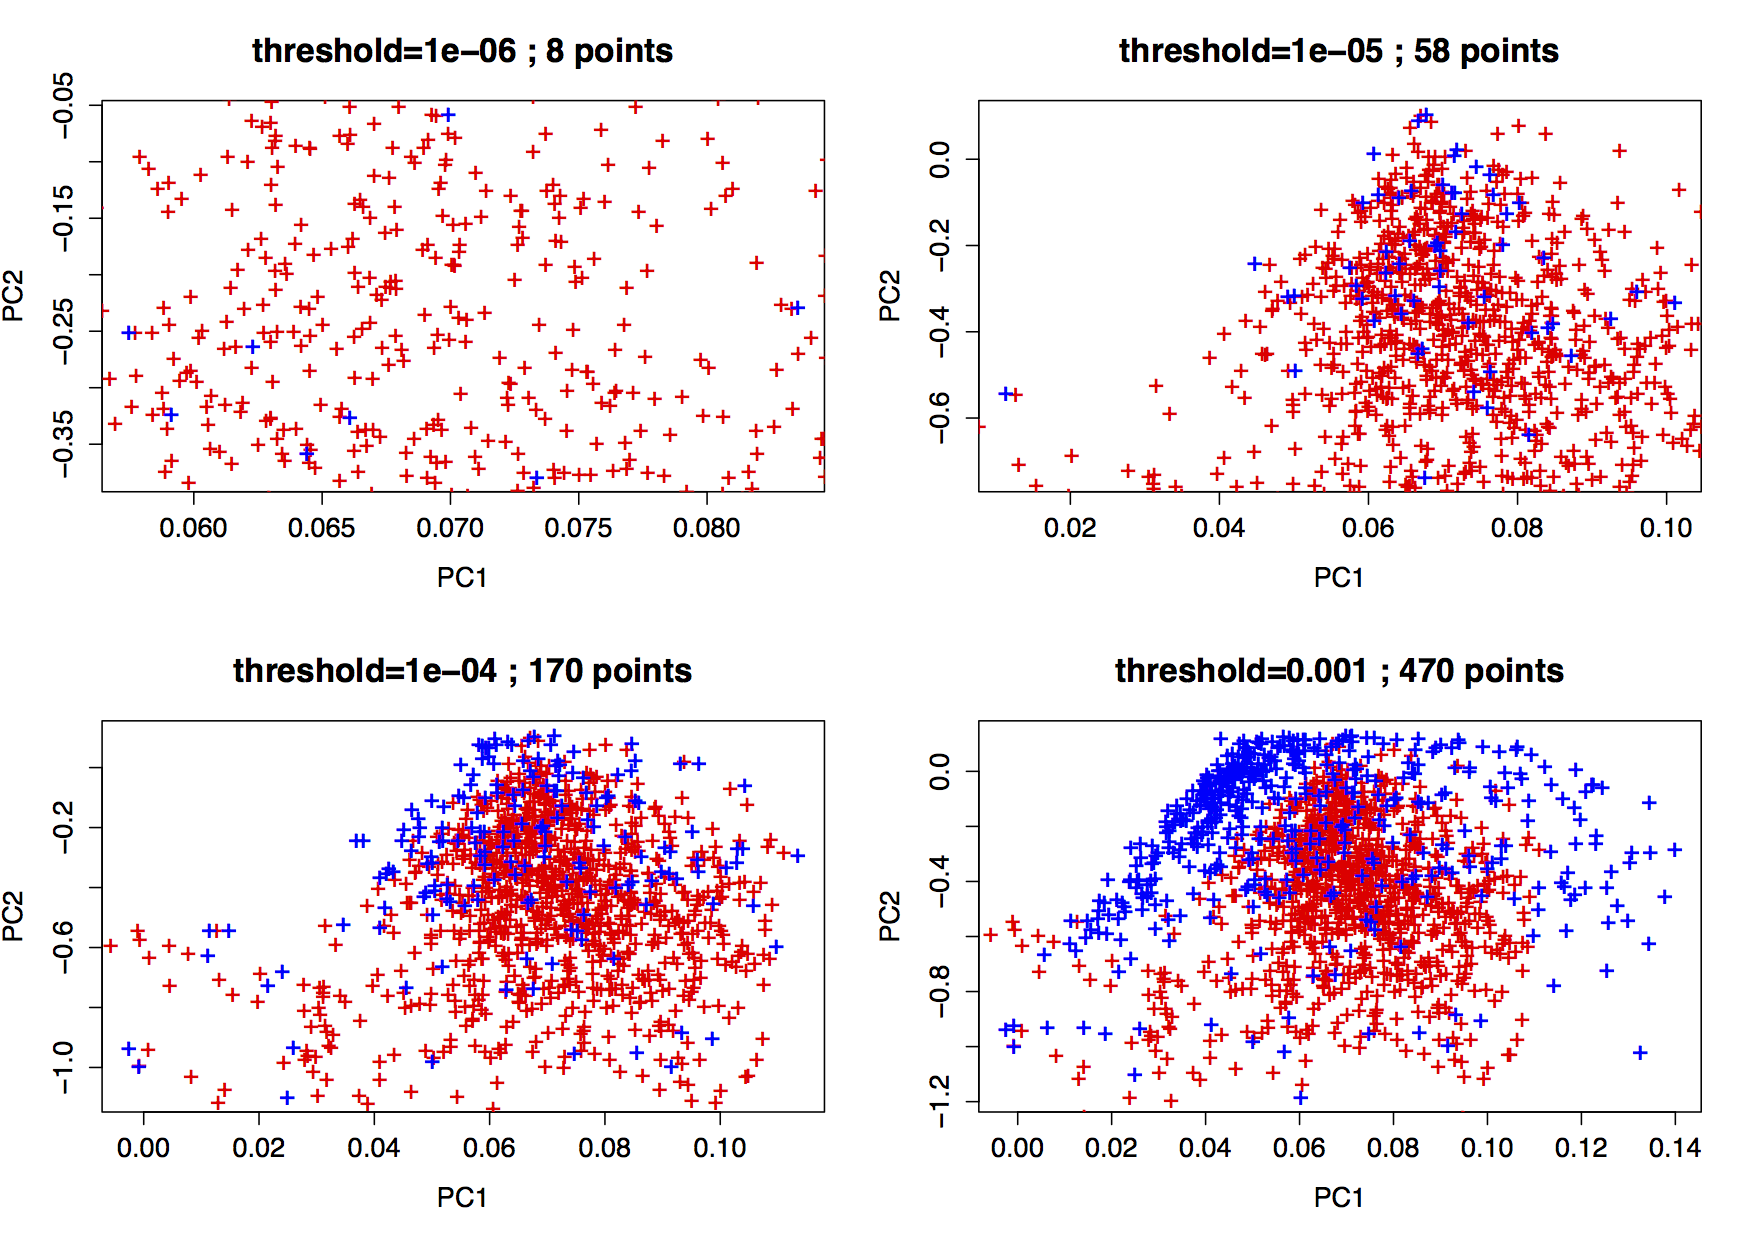
\includegraphics[width=\textwidth]{Figures/PartII/Modeling/UrbanGrowth/pcaDiff_thresholds}
\caption[Precise calibration of the model]{\textbf{Calibration of the model.} The principal component analysis is conducted to maximize the spread of the differences between real data and model output, i.e. on the set $\{\left|R_i - M_j\right|\}$ where $R_i$ is the set of real points, $M_j$ the set of model outputs. We select then the overlapping cloud at threshold $\theta$, by taking models output closer to real point cloud than $\theta$ in the (PC1,PC2) plan.}
\label{fig:densitycalib}
\end{figure}
%%%%%%%%%%%%%%







%%%%%%%%%%%%%%%%%%%%%%%%
\section*{Discussion}


more refined model : thresholded aggregation and diffusion (distance to center for diffusion, maximum density for aggregation)

\paragraph{Calibration refinement and Targeted Exploration}

We plan in further work to extract the exact parameter space covering all real situations and provide interpretation of its shape (correlations between parameters). Its volume in different directions should give the relative importance of parameters.




We also use the parameter space exploration algorithm~\cite{10.1371/journal.pone.0138212} implemented in OpenMole, and obtain in Fig.~\ref{fig:densitypse} the lower bound in Moran-entropy plan, that unexpectedly exhibit a scaling relationship that we aim to explore further.

%%%%%%%%%%%%%
\begin{figure}
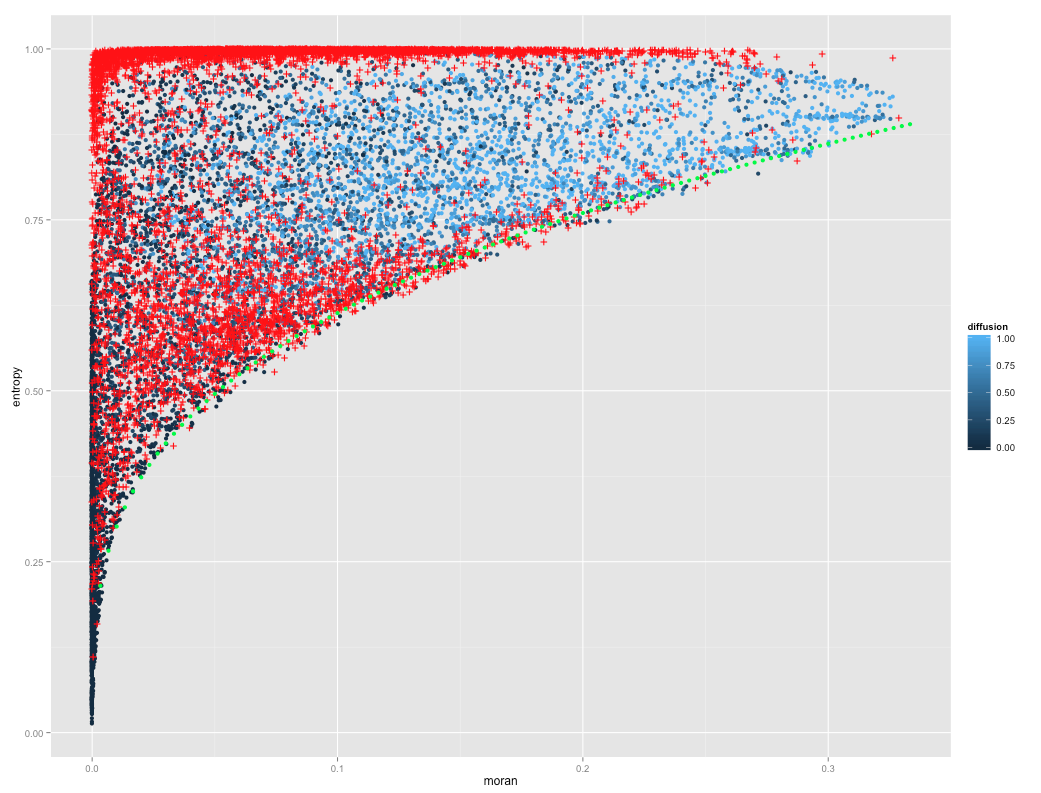
\includegraphics[width=\textwidth]{figures/Fig5.png}
\caption{\textbf{PSE exploration.} Scatterplotsof Moran against Entropy, with blue points obtained with LHS and red with PSE exploration. Lower bound is in green.}
\label{fig:fig5}
\end{figure}
%%%%%%%%%%%%%



%[possible development : application of Calibration Profile algo to check relative influence of parameters + ad hoc linear algebra on regression of 3.2.3 to do the same]


%%%%%%%%%%%%%%%%%%%%%%%%
%\subsection*{Thematic interpretation of growth behavior}

%We still need to interpret the positions of typical shapes within parameter space in order to confirm the thematic interpretation of parameters. Depending on results of calibration refinement, we may obtain necessary and sufficient parameters to explain growth at this scale and a corresponding interpretation.


% Dynamical calibration ?

% non stationary parameters ?



%%%%%%%%%%%%%%%%%%%%%%%%
\subsection*{Integration into a multi-scale growth model}

It could be possible to couple this model with a Gibrat (or Favaro-pumain) at Europa scale (macro) (with addition of consistence on migration constraints), where meso growth rates which were exogenous before are top-down determined, and bottom-up feedback is done through local aggregation level, influence importance of each area.


\cite{zhang2013identifying}






%%%%%%%%%%%%%%%%%%%%%%%%
\section*{Conclusion}


In conclusion, this first modeling step provide an accurately calibrated spatial urban growth model at the mesoscopic scale that can reproduce any European urban pattern in terms of urban form. Further work is needed for an interpretation of parameter influence and the determination of effective independent dimensions of the urban system at this scale. We will use this model for other purposes in the following.

% -> Accurately calibrated spatialized urban growth model, can reproduce any (european) urban pattern.
% -> interpretation of parameter influence ; effective independant dimensions of the urban system at this scale.




%%%%%%%%%%%%%%%%%%%%%%%%
\section*{Supporting Information}

% Include only the SI item label in the subsection heading. Use the \nameref{label} command to cite SI items in the text.


\subsection*{S1 Text}
\label{S1_Text}
{\bf Extended Model Exploration.}

\subsection*{S2 Text}
\label{S2_Text}
{\bf Semi-analytical Analysis.} Analytical and numerical developments of subsection~\ref{subsec:analytical}.



%\subsection*{S2 Text}
%\label{S2_Text}
%{\bf Extended empirical study of morphological indicators.} Contains maps of indicators for all Europe, statistical distributions of indicators, and some sensitivity analysis to grid size and typology parameters.


%%%%%%%%
% Potential supplementary material :
%  - sensitivity to neighborhood
%  - sensitivity of real values to window size



%%%%%%%%%%%%%%%%%%%%%%%%
%\section*{Acknowledgments}



\nolinenumbers

%\section*{References}
% Either type in your references using
% \begin{thebibliography}{}
% \bibitem{}
% Text
% \end{thebibliography}
%
% OR
%
% Compile your BiBTeX database using our plos2015.bst
% style file and paste the contents of your .bbl file
% here.
% 


\bibliographystyle{plos2015}
\bibliography{/Users/Juste/Documents/ComplexSystems/CityNetwork/Biblio/Bibtex/CityNetwork,biblio}















%%%%%%%%%%%%%% Tab template %%%%%%%%%%%%%%%%

%\begin{table}[!ht]
%\begin{adjustwidth}{-2.25in}{0in} % Comment out/remove adjustwidth environment if table fits in text column.
%\caption{
%{\bf Table caption Nulla mi mi, venenatis sed ipsum varius, volutpat euismod diam.}}
%\begin{tabular}{|l|l|l|l|l|l|l|l|}
%\hline
%\multicolumn{4}{|l|}{\bf Heading1} & \multicolumn{4}{|l|}{\bf Heading2}\\ \hline
%$cell1 row1$ & cell2 row 1 & cell3 row 1 & cell4 row 1 & cell5 row 1 & cell6 row 1 & cell7 row 1 & cell8 row 1\\ \hline
%$cell1 row2$ & cell2 row 2 & cell3 row 2 & cell4 row 2 & cell5 row 2 & cell6 row 2 & cell7 row 2 & cell8 row 2\\ \hline
%$cell1 row3$ & cell2 row 3 & cell3 row 3 & cell4 row 3 & cell5 row 3 & cell6 row 3 & cell7 row 3 & cell8 row 3\\ \hline
%\end{tabular}
%\begin{flushleft} Table notes Phasellus venenatis, tortor nec vestibulum mattis, massa tortor interdum felis, nec pellentesque metus tortor nec nisl. Ut ornare mauris tellus, vel dapibus arcu suscipit sed.
%\end{flushleft}
%\label{table1}
%\end{adjustwidth}
%\end{table}


%%%%%%%%%%%%% Fig. Template %%%%%%%%%%%%%%%%%

%\begin{figure}[h]
%\caption{{\bf Figure Title first bold sentence Nulla mi mi, venenatis sed ipsum varius, volutpat euismod diam.}
%Figure Caption Proin rutrum vel massa non gravida. Quisque tempor sem et dignissim rutrum. A: Lorem ipsum dolor sit amet. B: Consectetur adipiscing elit.}
%\label{fig1}
%\end{figure}




%%%%%%%%%%%%%% Eq. Template %%%%%%%%%%%%%%%%%

%\begin{equation}\label{eq:schemeP} 
%D_{coll} = \frac{D_f+\frac{[S]^2}{K_D S_T} D_S} {1+\frac{[S]^2}{K_D S_T}}, 
%D_{sm} = \frac{D_f+ \frac{[S]}{K_D} D_S}{1+\frac{[S]}{K_D}},
%\end{equation}





\end{document}

